\documentclass[10pt, a4paper,titlepage]{article}

\usepackage{graphicx}
\usepackage{tabularx}
\usepackage{listings}
\usepackage[normalem]{ulem}
\usepackage{caption}
\usepackage[bottom]{footmisc}
\usepackage{textcomp}
\usepackage{amsmath}

\begin{document}
\begin{titlepage}
\title{Project Plan Document\\Version 1.0}
\author{Emanuele Ricciardelli (mat. 875221) \and Giorgio Tavecchia (mat. 874716) \and Francesco Vetr\'o (mat. 877593)}
\begin{figure}
\begin{center}

\includegraphics{/home/francesco/git/Project_SE2_RTV/Project_Plan/PP_images/logopolimi.png}
\caption{Politecnico di Milano}
\label{fig:logo}
\end{center}
\end{figure}
\maketitle
\end{titlepage}
\tableofcontents
\pagebreak
\section{Introduction}
\subsection{Purpose and scope}
The purpose of this document, the Project Plan, is to analyze the complexity of the PowerEnJoy system in order to make a more accurate prediction of the costs and efforts necessary for the development of all the components of the system.
These data will then be useful to define budget, schedule and subdivision of resources and tasks within the team.
This document will be structured in 3 macro parts:
\begin{itemize}
\item The first section will deal with the analysis necessary to define an estimate of the size of the project, in function of lines of code, as well as the cost / effort. This analysis will be conducted in terms of Function Points and COCOMO II approach.
\item The second section will present a schedule for the project so as to ensure a proper distribution of tasks and times in order to achieve all of the system requirements, implementation and testing aspects.
\item In the third section we will discuss about risk management, through an analysis of possible problems that may arise during the development and the applicable remedies.
\end{itemize}•
\subsection{Definitions and abbreviations}
\begin{itemize}
\item RASD: Requirement Analysis and Specification Document.
\item DD: Design Document
\item ITPD: Integration Test Plan Document
\item PM: person-months
\item KSLOC: kilo-source lines of code
\end{itemize}
\subsection{Reference documents}
\begin{itemize}
\item Specification document: Assignments AA 2016-2017.pdf
\item RASD Version 1.1    
\item DD Version 1.1
\item ITPD Version 1.0
\item Project planning example document.pdf
\item Function Point Languages Table: \emph{http://www.qsm.com/resources/function-point-languages-table}
\end{itemize}
\section{Project size, cose and effort estimation}
This section will focus on providing an estimate of the size of the system that will be, as well as costs and development efforts.
Regarding the estimate of the size of the future system, we will make use of Function Point which will allow us to make an estimate based on the features that the system will have to offer.
Concerning the estimated costs and effort related to the development, we will make use of COCOMO II and we will integrate the results previously obtained.
\subsection{Size estimation: function points}
In this chapter we will face an approach through Function Point in order to estimate the size of the system to be developed, using as a unit of measurement the KSLOC.
In particular, we are going to make a calculation of all the Function Points of the system, by the following equation:
\begin{center}
UFP = $\sum$ (\# elements of a given type $\times$ weight)
\end{center}
The possible types of elements affecting the expression concern:
\begin{itemize}
\item Data structure;
\item Inputs and outputs;
\item Inquiries;
\item External Interface.
\end{itemize}
We provide a definition for each of them in the relevant section.
While, with respect to the definition of the weights, we are going to use the following table, which allows us to define, for each element, the weight as a function of the inherent complexity of its implementation.
\begin{table}[h]
\caption{Complexity weight}
\begin{tabularx}{\textwidth}{|>{\hsize=.4\hsize}X|>{\hsize=.2\hsize}X|>{\hsize=.2\hsize}X|>{\hsize=.2\hsize}X|}
\hline
Function type & Low & Average & High\\ 
\hline
Internal Logic Files & 7 & 10 & 15\\
\hline
External Interface Files & 5 & 7 & 10\\
\hline
External Inputs & 3 & 4 & 6\\
\hline
External Inquiries & 3 & 4 & 6\\
\hline
External Outputs & 4 & 5 & 7\\ 
\hline
\end{tabularx}
\end{table}
\subsubsection{Internal Logic Files (ILFs)}
With Internal Logic Files we define internal data generated by
the system, and used and maintained by it. This set contains homogenous data handled by the system, composed by all the data structure saved in the DBMS.
In the list below we list the tables which compose our database. They fill the Internal Logic Files set.
\begin{itemize}
\item User(\underline{Password}, email, name, surname,drivingLicenseNumber)
\item Reservation(\underline{ID,userPassword,licensePlateCard}, date,startingTime,endingTime)
\item Car(\underline{licensePlate}, model)
\item MaintenanceRecord(\underline{ID},description,date, licensePlate)
\item Sensor(\underline{ID}, licensePlate)
\item ExtraInRes(\underline{ID, IDextra, IDreservation})
\item Extras(\underline{ID}, type, value)
\item Payment(\underline{prog\_number, IDReservation}, pending, date)
\item Ride(\underline{ID}, IDReservation, startingTime, endingTime, bill, lastBatteryLevel,date, startingSafeArea, endingArea)
\item Ticket(\underline{IDTicket, IDRide}, date)
\item Area(\underline{ID}, position)
\item SafeArea(\underline{IDArea})
\item UnsafeArea(\underline{IDArea})
\item PowerGrid(\underline{ID}, capacity, IDSafeArea)
\item BonusMalus(\underline{ID}, amount, description)
\item AssignedBonusMalus(\underline{IDRide, IDBonusMalus})
\end{itemize}
With respect to the previous table of complexity weight, we decide to assign a \emph{LOW} level to those tablet that are composed by a small number of attributes, while we define as \emph{AVERAGE} level of complexity tables such as Reservation that is derived from the interaction of multiple tables. For the same reason, but with an higher level of complexity, we assign to the Ride table the \emph{HIGH} level.
\begin{table}[h]
\caption{ILFs}
\begin{tabularx}{\textwidth}{|>{\hsize=.5\hsize}X|>{\hsize=.25\hsize}X|>{\hsize=.25\hsize}X|}
\hline
ILF & Complexity Level & FPs\\ 
\hline
User & Low & 7\\
\hline
Reservation & Avg & 10\\
\hline
Car & Low & 7\\
\hline
Maintenance Record & Low & 7\\
\hline
Sensor & Low & 7\\
\hline
ExtraInRes & Low & 7\\
\hline
Extras & Low & 7\\
\hline
Payment & Low & 7\\
\hline
Ride & High & 15\\
\hline
Ticket & Low & 7\\
\hline
Area & Low & 7\\
\hline
Safe Area & Low & 7\\
\hline
Unsafe Area & Low & 7\\
\hline
Power Grid & Low & 7\\
\hline
BonusMalus & Low & 7\\
\hline
AssignedBonusMalus & Low & 7\\
\hline
& TOT & 123\\
\hline
\end{tabularx}
\end{table}
\pagebreak
\subsubsection{External Interface Files (EIFs)}
With External Interface Files we identify a set of data used by the PowerEnJoy system that are not stored in it but provided and handled by external companies.
With respect to the PowerEnJoy service, the external data are provided by Google Services and in particular by Google Maps.
The services above, are used by our system making use of the API provided by Google itself. Features requiring their use are as follows:
\begin{itemize}
\item Provide directions, given the current position of a car, to a charging station.
\end{itemize}
This functionality is implemented in the Money-Saving option, in which the user is able to enter their destination and the system returns the location of the nearest charging station to the destination, providing at the same time a uniform distribution of cars in the city; this position will later be used by the API to calculate the optimal route and return there.
Given the complexity of the operations involved (especially those linked to the uniform distribution of cars in the city) we identify this feature as a \emph{AVG} complexity.
\begin{table}[h]
\caption{ELFs}
\begin{tabularx}{\textwidth}{|>{\hsize=.5\hsize}X|>{\hsize=.25\hsize}X|>{\hsize=.25\hsize}X|}
\hline
ELF & Complexity Level & FPs\\ 
\hline
Money saving option & Avg & 7\\
\hline
\end{tabularx}
\end{table}
\pagebreak
\subsubsection{External Inputs (EIs)}
With External Input we identify a set of elementary operation to elaborate data coming from
the external environment.
As defined in previous documents, our system interfaces with a number of clients aimed at different types of users, in particular we will have functionality addressed to users of car sharing service, the maintenance system and the payment system.
In particular for each of them we will provide the following functionalities:
\begin{itemize}
\item Users of the car sharing service:
\subitem - Login/Logout: the login and logout are key features to our system but there are translated into simple queries on the database, which is why the level of complexity is \emph{LOW}.
\subitem - Registration: the registration system is also based on a number of queries on the database, to which, however, are added a series of controls regarding the information entered, the validity of the license provided and the accuracy of data relating to the method of payment chosen. Despite this, it remains a \emph{LOW} complexity.
\subitem - Reserve a car: booking a car is a complex operation that requires a series of queries, followed by several controls both the user (Eg. check if it is suspended) and the selected car (Eg. make sure it is available) and finally a communication with the vehicle to inform the reservation. the multiplicity of the transactions underlying the achievement of this feature allows us to indicate it as a \emph{AVG} complexity.
\subitem - Delete a reservation: linear operation and \emph{LOW} complexity since it corresponds to the simple closure of the reservation and the consequent reflection on the database.
\subitem - Extend a reservation: the operations involved are the same as the \emph{Delete a reservation}, the only addition corresponds to the operations necessary to register the payment due to the extension itself. For this reason, the level of complexity is \emph{LOW}.
\subitem - Start a ride: the operation to \emph{start a ride} requires an exchange of information between the car and the system, in particular the operation can begin when the system validates the unlock code used on the car and the engine is ignited. The underlying operations of this feature affect several components that are going to instantiate different entity in the database. For these reason we define an \emph{AVG} complexity.
\subitem - End a ride: like the previous functionality, are involved different components and entities in the database. the complexity, also in this case, is \emph{HIGH} because the system does not only apply queries on the database but compute all the necessary element to end a ride, like computing the payment and various discounts. This functionality is more complex than “Start a Ride” because in order to fulfill its task, it requires the product of more subprocesses like computing the total amount, performing the payment instantiation, unreserved the car and so on.
\subitem Report a issue: reporting a problem to a car, it may seem a simple task since it requires only the creation of a new “record maintenance”, but underneath  resides the management of the whole reservation or ride that interested the machine. for this reason the average complexity is \emph{AVG}. 
\item Maintenance system:
\subitem - Update a record about a car: the status update concerning a record of a car by the maintenance is a simple task that requires only to update tuples in the database related to the reported car. The complexity is \emph{LOW}.
\item Payment system:
\subitem - Update payment informations: just as in the case of update by maintenance, the only operation involved  is upgrading tuples in the database for a specified payment. The complexity is \emph{LOW}.
\end{itemize}
\begin{table}[h]
\caption{EIs}
\begin{tabularx}{\textwidth}{|>{\hsize=.5\hsize}X|>{\hsize=.25\hsize}X|>{\hsize=.25\hsize}X|}
\hline
EI & Complexity Level & FPs\\ 
\hline
Login/Logout & Low & 3$\times$2=6\\
\hline
Registration & Low & 3\\
\hline
Reserve a Car & Avg & 4\\
\hline
Delete reservation & Low & 3\\
\hline
Extend reservation & Low & 3\\
\hline
Start ride & Avg & 4\\
\hline
End ride & High & 6\\
\hline
Report issue & Avg & 4\\
\hline
Update record car & Low & 3\\
\hline
Update payment information & Low & 3\\
\hline
& TOT & 39\\
\hline
\end{tabularx}
\end{table}
\pagebreak
\subsubsection{External Inquiries (EQs)}
With External Inquiries we define a set of elementary operation that involves input and output operations. With regard to this definition and using the previous subdivision related to different users of the system, we provide the following functionalities:
\begin{itemize}
\item Users of the car sharing service:
\subitem - Retrieve information about his reservation
\subitem - Retrieve unlock code: the previous two steps possess the same level of complexity as they are the result of a simple query to the database, for this reason, is associated to them a \emph{LOW} complexity.
\subitem - Retrieve payment history: since the payment-related information is obtained through analysis of all the costs relating to reservations and ride (e.g. the extension of a reservation or the application of discounts), the complexity of this operation is \emph{AVG}.
\subitem - View available cars: the identification of available cars is the result of an analysis of the non-reserved cars or currently in use /in  maintenance. For this reason, the complexity is \emph{LOW}.
\item Maintenance system:
\subitem - Retrieve a list of reported issue: as well as retrieving information associated with a reservation, cited above, retrieving reports is a simple task, result of an equally simple database query. Complexity \emph{LOW}. 
\end{itemize}
\begin{table}[h]
\caption{EQs}
\begin{tabularx}{\textwidth}{|>{\hsize=.5\hsize}X|>{\hsize=.25\hsize}X|>{\hsize=.25\hsize}X|}
\hline
EQ & Complexity Level & FPs\\ 
\hline
Retrieve reservation info & Low & 3\\
\hline
Retrieve unlock code & Low & 3\\
\hline
Retrieve payment history & Avg & 4\\
\hline
View available cars & Low & 3\\
\hline
Retrieve list of reported issues & Low & 3\\
\hline
& TOT & 16\\
\hline
\end{tabularx}
\end{table}
\pagebreak
\subsubsection{External Outputs (EOs)}
With External Output we define functionalities that our system perform and generate data to the output. 
With respect to this definition, we can define the following functionalities:
\begin{itemize}
\item Notify a user for the correct registration;
\item Notify a user that a reservation has been performed;
\item Notify a user if the car reserved is no longer available;
\item Notify a user for the payment of a ride;
\item Notify the maintenance system if a new issue is reported;
\item Notify the payment system if a new debt is created.
All the notifications listed above are considered simple and for this reason the \emph{LOW} complexity.
\end{itemize}
\begin{table}[h]
\caption{EOs}
\begin{tabularx}{\textwidth}{|>{\hsize=.5\hsize}X|>{\hsize=.25\hsize}X|>{\hsize=.25\hsize}X|}
\hline
EO & Complexity Level & FPs\\ 
\hline
Notify correct registration & Low & 4\\
\hline
Notify performed reservation & Low & 4\\
\hline
Notify car no longer available & Low & 4\\
\hline
Notify payment & Low & 4\\
\hline
Notify new issue & Low & 4\\
\hline
Notify new debt & Low & 4\\
\hline
& TOT & 24\\
\hline
\end{tabularx}
\end{table}
\pagebreak
\subsubsection{Overall estimation}
Given the following summary table:
\begin{table}[h]
\caption{Summary}
\begin{tabularx}{\textwidth}{|>{\hsize=.5\hsize}X|>{\hsize=.5\hsize}X|}
\hline
Function type & Value\\ 
\hline
Internal Logic Files & 123\\
\hline
External Interface Files & 7\\
\hline
External Inputs & 39\\
\hline
External Inquiries & 16\\
\hline
External Outputs & 24\\
\hline
Total & 209\\
\hline
\end{tabularx}
\end{table}
\linebreak
\begin{center}
LOC=AVC$\times$number of function points
\end{center}
Considering Java Enterprise Edition as the development platform, we can assign the value AVC  following the Function Point Language Table linked in the document references.
For the average number of SLOC AVC is equal to 46: 
\begin{center}
SLOC= 209$\times$46= 9614
\end{center}
For the computing an upperbound for the number of SLOC AVC is equal to 67:
\begin{center}
SLOC=209$\times$67=14003
\end{center}
\subsection{Cost and effort Estimation: COCOMO II}
In this section, as previously expressed in the purpose of the document, we will use the COCOMO II approach in order to estimate cost and effort needed to develop the PowerEnJoy system. In particular we will focus on a Post-Architecture approach since we have already detailed informations about the different phases of development, and so we can achieve a more accurate cost estimate.
We now provide an accurate analysis of all the elements needed to perform the following effort equation:
\begin{center}
PM=A$\times$Size$^E\times\prod_{1<=i<=n}EM_i$
\end{center}
In particular, the meaning of the coefficients is the following:
\begin{itemize}
\item A: It’s an approximation of the productivity constant in PM/KSLOC. This coefficient is standardly set to 2.94;
\item Size: is the estimated size of the project in KSLOC, provided in the previous chapter;
\item $EM_i$: effort multiplier, derived for each cost driver;
\item E: is an aggregation of five Scale Factors.
\end{itemize}
\subsubsection{Scale factors}
The first parameter that we will estimate is \emph{E}, obtained by the following equation, a function of scale factors that we will soon identify.
\begin{center}
E=B+0.01$\times\sum_{1<=j<=5}SF_j$
\end{center}
Where B is set to 0.91, as an empirically-proven quantity for COCOMO II.
Regarding $SF_j$, each member of the summation is equivalent to a coefficient of the following table, chosen in function of the range of verylow-extrahigh values, characteristic of each of them.
\begin{figure}[h]
\begin{center}
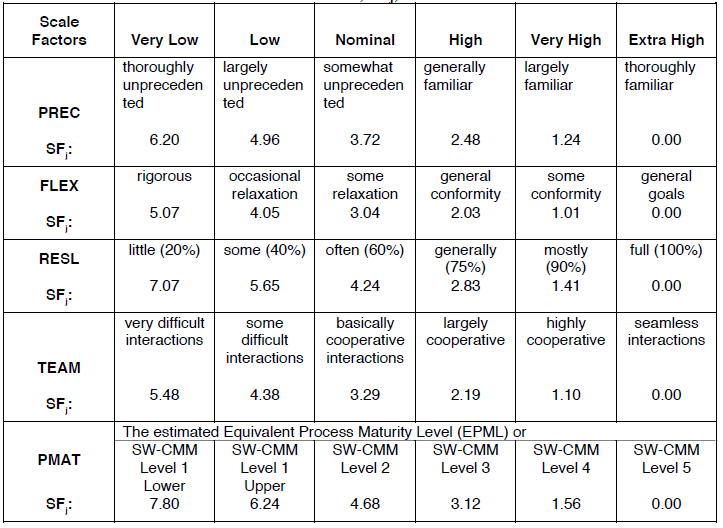
\includegraphics[width=\textwidth, height=0.8\textheight, keepaspectratio]{/home/francesco/git/Project_SE2_RTV/Project_Plan/PP_images/scale_factors.png}
\caption{Scale Factors}
\label{fig:scale}
\end{center}•
\end{figure}
\pagebreak
For each of these factors, we will now provide a definition and the reasoning behind the chosen value:
\begin{itemize}
\item \underline{\textbf{Precedentedness (PREC)}}:  The value of this coefficient decreases much higher is the degree of experience that the team presents in respect of a similar project. In particular, our experience level is \emph{LOW} because we have not previously participated in the development of systems of this size.
\item \underline{\textbf{Development Flexibility (FLEX)}}: The degree of development flexibility reflects the flexibility that the project can presents regarding the requirements and objectives on which it was founded. The PowerEnJoy system has been defined in relation to requirements for the car sharing service that have stiffness from the point of view of the required functionality, with little choice margin, while from the architectural point of view is more flexible since there are no systems legacy to which it is necessary to integrate, but, at the same time, the type of service involves the development of an architecture able to ensure certain levels of operations. For this reason, we assign a \emph{NOMINAL} value.
\item \underline{\textbf{Risk Resolution (RSL)}}: This factor reflects the ability of the development team to recognize and react promptly to the risks and problems that it could be encountered along the development. Also in relation to the same subject discussed in detail in the final chapter of this document, we assign the value \emph{HIGH}.
\item \underline{\textbf{Team Cohesion (TEAM)}}: The Team Cohesion scale factor accounts for the sources of project turbulence and entropy because of difficulties in synchronizing the project’s stakeholders: users, customers, developers etc. These difficulties may arise from differences in stakeholder objectives and cultures, difficulties in reconciling objectives and developer’s lack of experience and familiarity in operating as a team. With respect to this definition we can assign a \emph{VERY HIGH} level, since the development team is collaborative and open to dialogue.
\item \underline{\textbf{Process Maturity (PMAT)}}: This factor is directly linked with the CMMI index, in particular, related to our system, the development project has been properly managed, planned and executed with stakeholders involved and resources rightly distributed. For this rationale, we assign a Level 2, so a \emph{NOMINAL} factor. 
\end{itemize}
\pagebreak
We can now compute the previously presented equation:
\begin{table}[h]
\caption{Scale Factor}
\begin{tabularx}{\textwidth}{|>{\hsize=.5\hsize}X|>{\hsize=.25\hsize}X|>{\hsize=.25\hsize}X|}
\hline
Scale Factor & Factor & Value\\ 
\hline
Precedentedness (PREC) & Low & 4.96\\
\hline
Development Flexibility (FLEX) & Nominal & 3.04\\
\hline
Risk Resolution (RSL) & High & 2.83\\
\hline
Team Cohesion(TEAM) & Very High & 1.10\\
\hline
Process Maturity (PMAT) & Nominal & 4.68\\
\hline
&  & 16.61\\
\hline
\end{tabularx}
\end{table}
\linebreak
Using the previously defined equation:
\begin{center}
E= 0.91+0.01$\times$16.61=1.0761
\end{center}
\subsubsection{Cost drivers}
\end{document}


